% !Mode:: "TeX:UTF-8"
\chapter{面向博物馆导览的数字人智能交互设计框架分析}

本文提出\textbf{面向博物馆导览的数字人智能交互设计框架}。该框架指向一种面向真实参观过程的数字人导览组织方法：以展品知识为内容基础，以参观现场中的空间位置、用户关注点与会话进程为情境约束，以数字人的语言、动作、视线和语音节奏为外显媒介，使系统能够持续判断此刻应讲什么、讲到什么深度、如何承接用户问题、何时推进或切换主题，并将导览意图转化为观众能够感知和跟随的交互过程。在这一框架中，智能交互并不只等同于生成回答，而是体现为内容组织、情境维护与外显引导之间的协同。

基于这一定义，本文将前文提出的三个研究问题进一步转化为框架维度：针对\textbf{展品知识信息复杂，难以交互化呈现}的问题，框架设置面向导览推进的叙事组织机制，用于把展品知识组织为可分层进入、可持续追问、可回收推进的讲解路径；针对\textbf{导览情境断裂，参观状态难以把握}的问题，框架设置面向现场导览的情境编排机制，用于维护当前展品、空间位置、参观阶段、用户关注点与会话进程，使导览内容始终落在具体现场条件之中；针对\textbf{数字人呈现脚本化，注意力引导弱}的问题，框架设置面向导览感知的外显引导机制，用于将导览意图转化为动作、视线、语音节奏与角色表达等可被观众感知的引导线索。三者共同构成面向博物馆导览的数字人智能交互设计框架，使数字人从单纯播报与问答回应，转向能够组织内容、维护情境并外显引导意图的主动导览主体。

\section{面向导览推进的叙事组织机制}
面向导览推进的叙事组织机制关注导览内容如何在开放交互中被组织为可持续展开的讲解过程。博物馆导览所面对的是一种伴随参观移动、注意力转移与理解逐步深入而不断展开的学习过程。数字人要在这一过程中承担导览角色，核心在于把展品知识组织成能够被进入、被承接、被延展并最终被收束的讲解结构，使每一轮回应都处在整体导览脉络之中，并持续服务于连贯的理解推进。前文中提出的层级叙事单元、追问路径与回收策略，正是这一机制的基础依据。
如图\ref{fig-conversation-mechanism}所示，叙事组织机制通过分层组织、路径铺陈与主线回收三个环节共同支撑导览推进。

\begin{figure}[htbp]
    \centering
    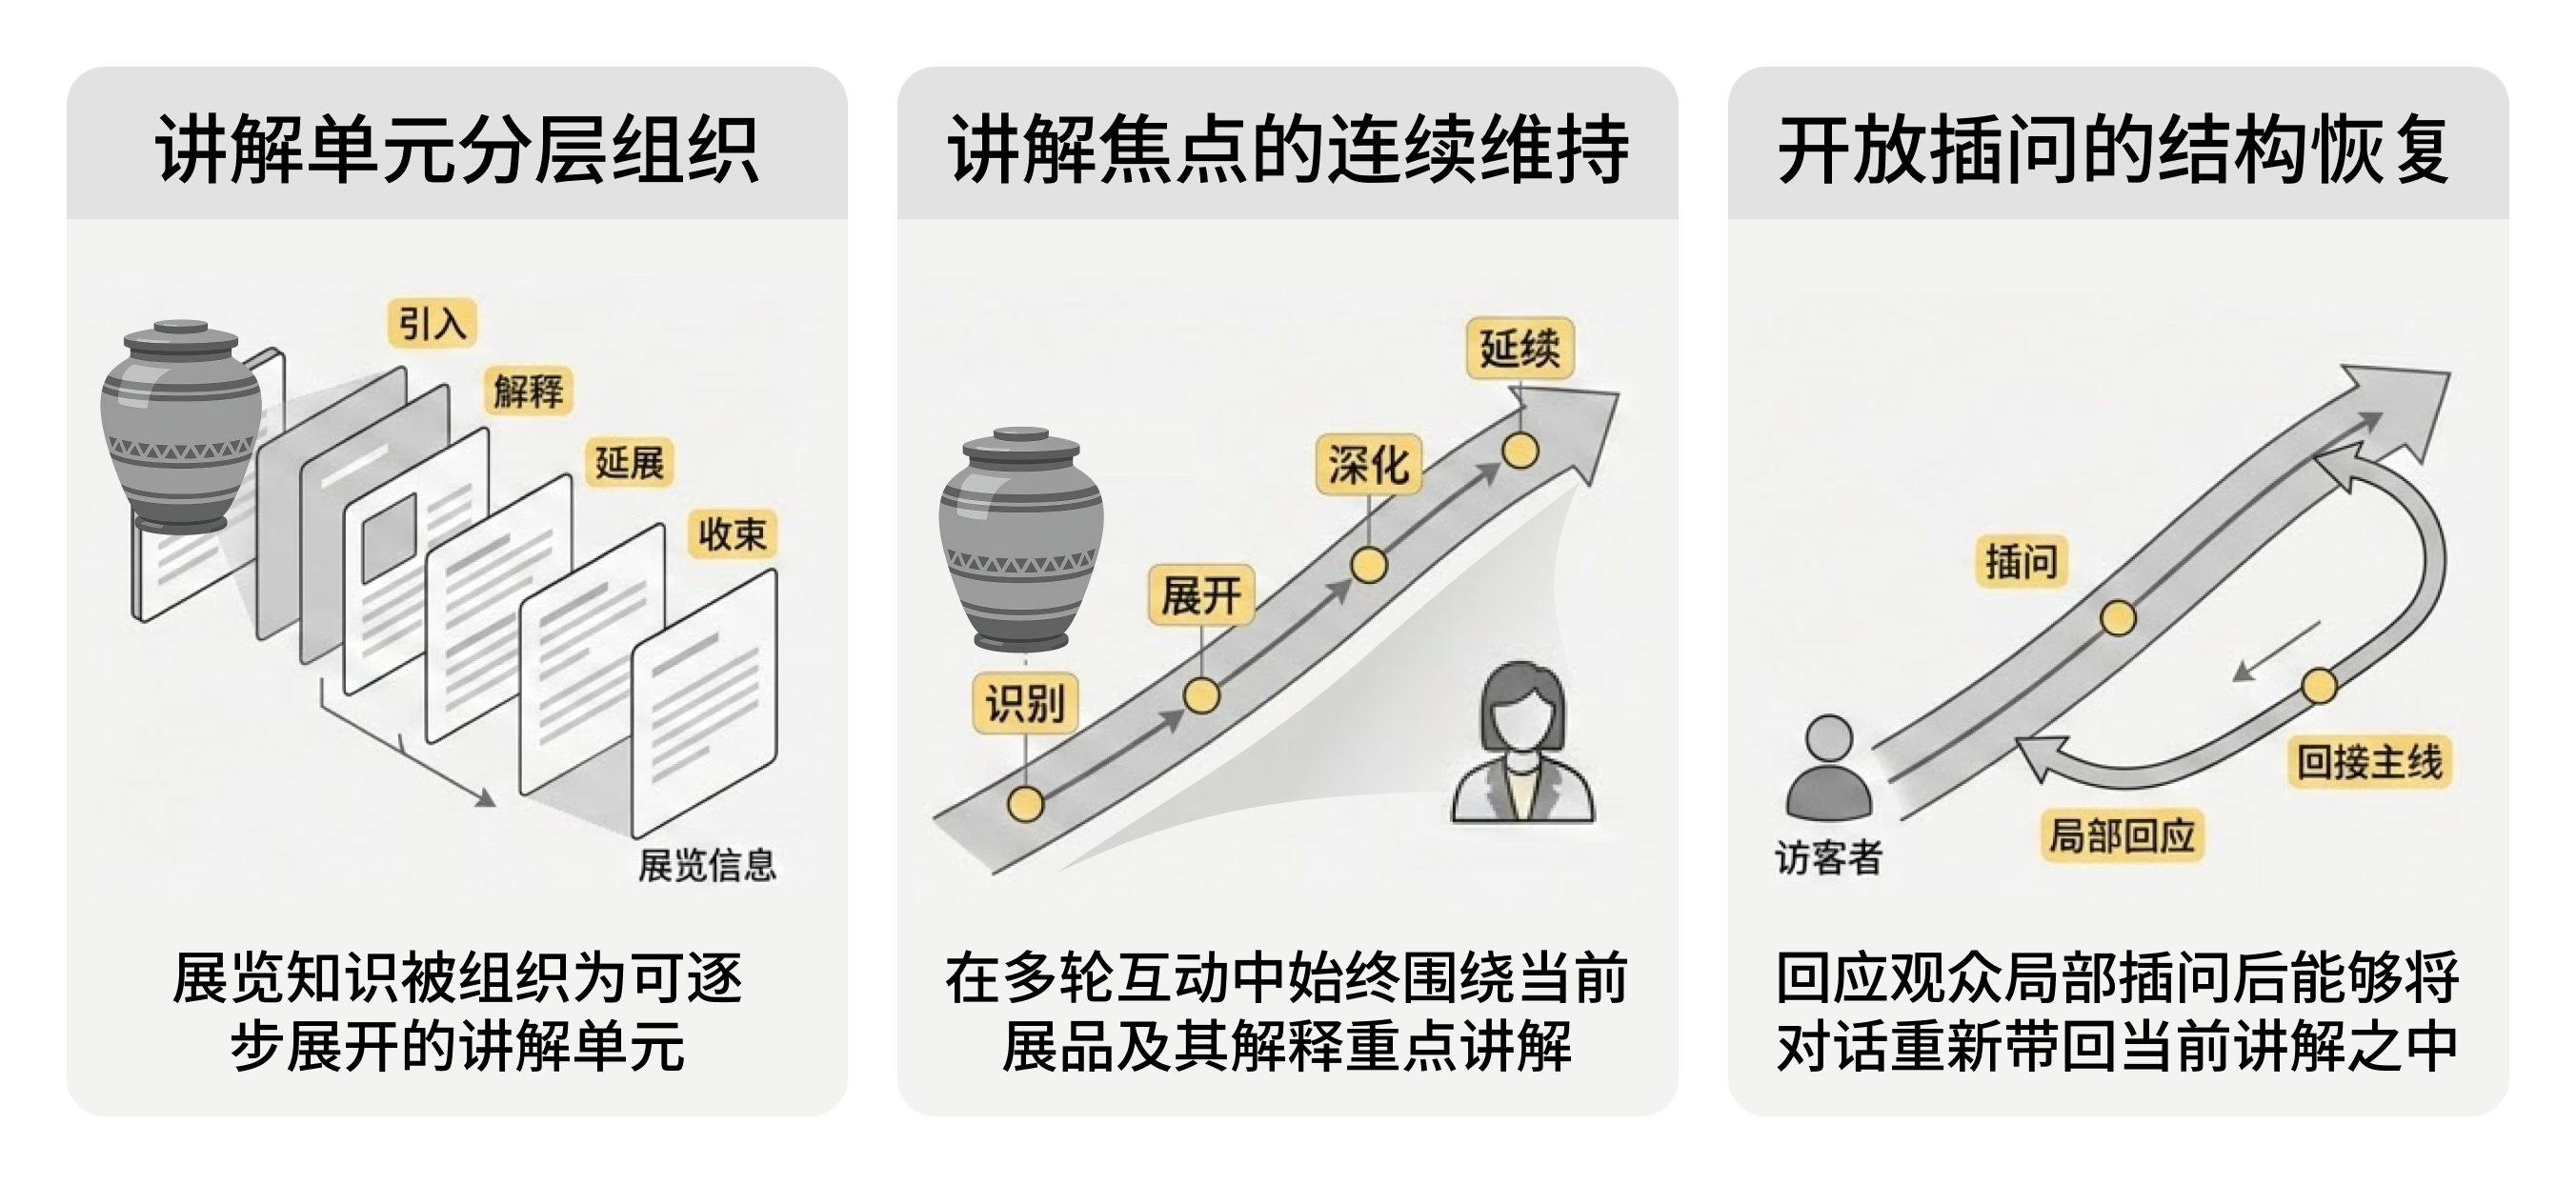
\includegraphics[width=\textwidth]{figure/figs/conversation.png}
    \caption{面向导览推进的叙事组织机制示意图}
    \label{fig-conversation-mechanism}
\end{figure}

\subsection{讲解单元的分层组织}
在这一维度中，首先需要完成讲解单元的分层组织。展品知识进入导览过程时，应被整理为承担不同导览作用的叙事单元。例如，用于建立初步识别的引入性内容，用于解释背景与意义的展开性内容，用于延长兴趣和联结经验的延展性内容，以及用于重新聚焦主题的收束性内容。这样的组织方式使导览内容具有明确的层次和颗粒度，也使讲解从知识堆叠转化为可被调度、可被重组的叙事资源。数字人由此获得的是一套能够围绕学习推进被灵活编排的讲解材料。

\subsection{讲解焦点的连续维持}
在博物馆导览场景中，讲解需要围绕当前展品及其解释重点持续展开。讲解焦点的连续维持，是指系统在多轮互动过程中始终围绕当前讲解对象组织回应，使后续内容能够承接前文、贴合当前对象，并服务于同一讲解方向的逐步展开。通过这一机制，多轮互动能够在同一焦点下形成连续的解释链条，帮助观众围绕展品逐步建立理解。在实际参观过程中，观众往往会围绕同一展品提出不同层次的问题，例如历史背景、形式特征、工艺细节、文化含义及与周边展品的关联。讲解焦点的连续维持，使这些问题能够被组织进同一讲解线索之中，使讲解内容在对象一致的前提下持续补充、延展和深化，形成稳定的理解路径。借助这一机制，导览对话能够保持意义聚焦与线索连贯，从而提升现场讲解的连续性与跟随感。

\subsection{开放插问后的结构恢复}
在博物馆导览过程中，观众的提问往往带有即时性和开放性，常常会在讲解推进中插入局部追问、补充确认或临时转向。开放插问后的结构恢复，是指系统在回应观众插问后，能够将对话重新带回当前讲解线索之中，使局部偏离后的讲解继续围绕原有对象与解释重点展开。该机制关注的核心，是在保留互动开放性的同时维持讲解结构的整体连贯，使导览过程能够持续推进。对于导览任务而言，插问本身构成了理解深化的重要契机。观众可能在讲解过程中临时追问某一细节，也可能针对当前展品提出补充性问题。这类插问能够增强互动参与，但也容易使讲解内容停留在局部回应之中，削弱原有讲解线索的连续性。开放插问后的结构恢复，使系统能够在完成局部回应后重新收束讲解内容，将当前回答纳入原有讲解过程之中，继续围绕当前展品及其解释重点展开，从而保持讲解的整体方向与组织秩序。借助这一机制，对话式数字人展示能够在开放互动与导览连贯之间形成平衡。一方面，观众的即时问题可以被及时接住并得到回应，导览体验因此具有更强的参与性与可进入性；另一方面，讲解不会因局部插问而持续偏离，而是能够在回应之后重新回到当前讲解结构之中，维持解释链条的完整性与导览叙事的连续性。对于面向博物馆导览的对话式数字人展示而言，这一机制有助于提升多轮讲解中的可回收性，使开放式互动真正服务于讲解推进，而非消解讲解本身的组织结构。

因此，面向导览推进的叙事组织机制通过讲解单元的分层组织、讲解焦点的连续维持以及开放插问后的结构恢复，使数字人能够围绕参观者的理解过程持续展开讲解，并在真实场域中维持导览脉络的连续性、可进入性与可回收性。这样的组织结果也为后续情境状态的判断与展示线索的外显提供了可读取的语义基础，使叙事组织机制成为整个框架中导览推进得以成立的起点。根据后续对系统机制的映射，这一机制最终会落实为可供状态更新与展示调度读取的语义组织对象，承载当前轮的讲解目标、信息结构与潜在追问入口。

\section{面向现场导览的情境编排机制}
面向现场导览的情境编排机制关注导览如何围绕参观现场的具体条件被持续组织。博物馆中的导览活动始终发生在特定的参观进程之中：参观者带着既有兴趣、知识经验与注意取向进入展厅，在移动、停留、提问与观看中不断调整自己的理解路径；与此同时，展区位置、空间对象、互动关系与时间推进也持续改变导览发生的条件。前文引入的情境学习框架已经说明，博物馆学习受到个人、社会文化、物理情境及时间过程的共同影响，导览的有效性取决于它能否贴合这些具体条件展开。
如图\ref{fig-context-mechanism}所示，情境编排机制通过情境线索组织、现场状态更新与策略约束实现导览过程的持续编排。

\begin{figure}[htbp]
    \centering
    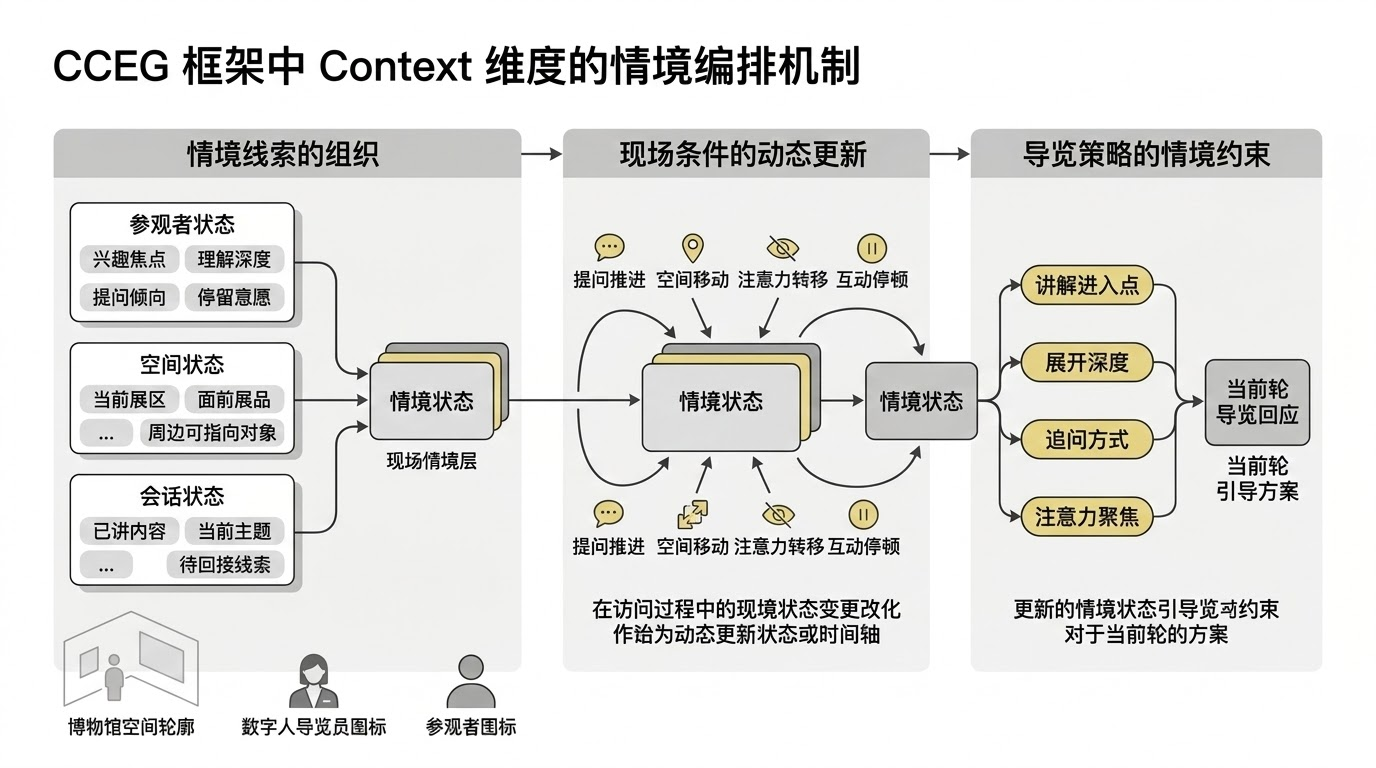
\includegraphics[width=\textwidth]{figure/figs/Context.png}
    \caption{面向现场导览的情境编排机制示意图}
    \label{fig-context-mechanism}
\end{figure}

\subsection{情境线索的组织}
基于此，情境编排机制需要先将现场导览中的关键条件组织为可判断的情境线索。本文将其概括为三类：其一是参观者状态，包括当前兴趣焦点、理解深度、提问倾向与停留意愿等，用以描述参观者此刻希望进入什么、已经理解到哪里；其二是空间状态，包括当前展区位置、正在面对的展品对象以及周边可被指向和比较的展示元素，用以描述导览发生在何处、围绕何物展开；其三是会话状态，包括既有讲解进度、当前主题焦点、尚未完成的解释线索与可被重新回接的内容节点，用以描述导览脉络已经推进到何种阶段。通过这样的组织，情境从附着于对话之外的背景材料转化为导览得以成立的现场条件。

\subsection{现场条件的动态更新}
这些情境线索还需要随着参观进程持续更新。博物馆导览具有明显的过程性特征：参观者会因为兴趣聚焦而连续追问，也可能因为疲劳、干扰或路径切换而中断原有节奏；空间对象会随着移动发生变化，讲解进入点也会随之调整；已经建立的背景解释会在后续互动中积累为新的理解前提。情境编排机制因此承担着对导览现场进行动态编排的任务，它需要根据提问内容、观看行为、空间转移与会话延续不断修正当前情境，使数字人所面对的始终是此时、此地、此人的具体参观状态。后文的闭环流程设计也体现了这一点：系统依据语义组织结果与用户反馈更新情境状态，并在此基础上调整讲解粒度、追问策略与路径维持方式。

\section{面向导览感知的外显引导机制}
\subsection{外显引导的框架定位}
如图\ref{fig-eg-mechanism}所示，在本文框架中，外显引导机制承担着将叙事组织与情境编排转化为可感知交互行为的作用。叙事组织机制形成导览内容的展开顺序、讲解层级与追问路径，情境编排机制维护当前展品、空间位置、用户关注点与导览进程，二者共同决定数字人在某一时刻应当表达的导览意图。外显引导机制进一步将这一导览意图落实到数字人的视线、手势、身体朝向、语音节奏与表达状态中，使观众能够通过可见、可听的多模态线索理解当前应关注什么、为什么继续听、何时可以提问以及导览正在如何推进。由此，外显引导成为连接系统内部导览决策与观众现场体验的关键环节，也使数字人的智能交互从文本回应延伸为具有方向感、节奏感和陪伴感的导览过程。

\begin{figure}[htbp]
    \centering
    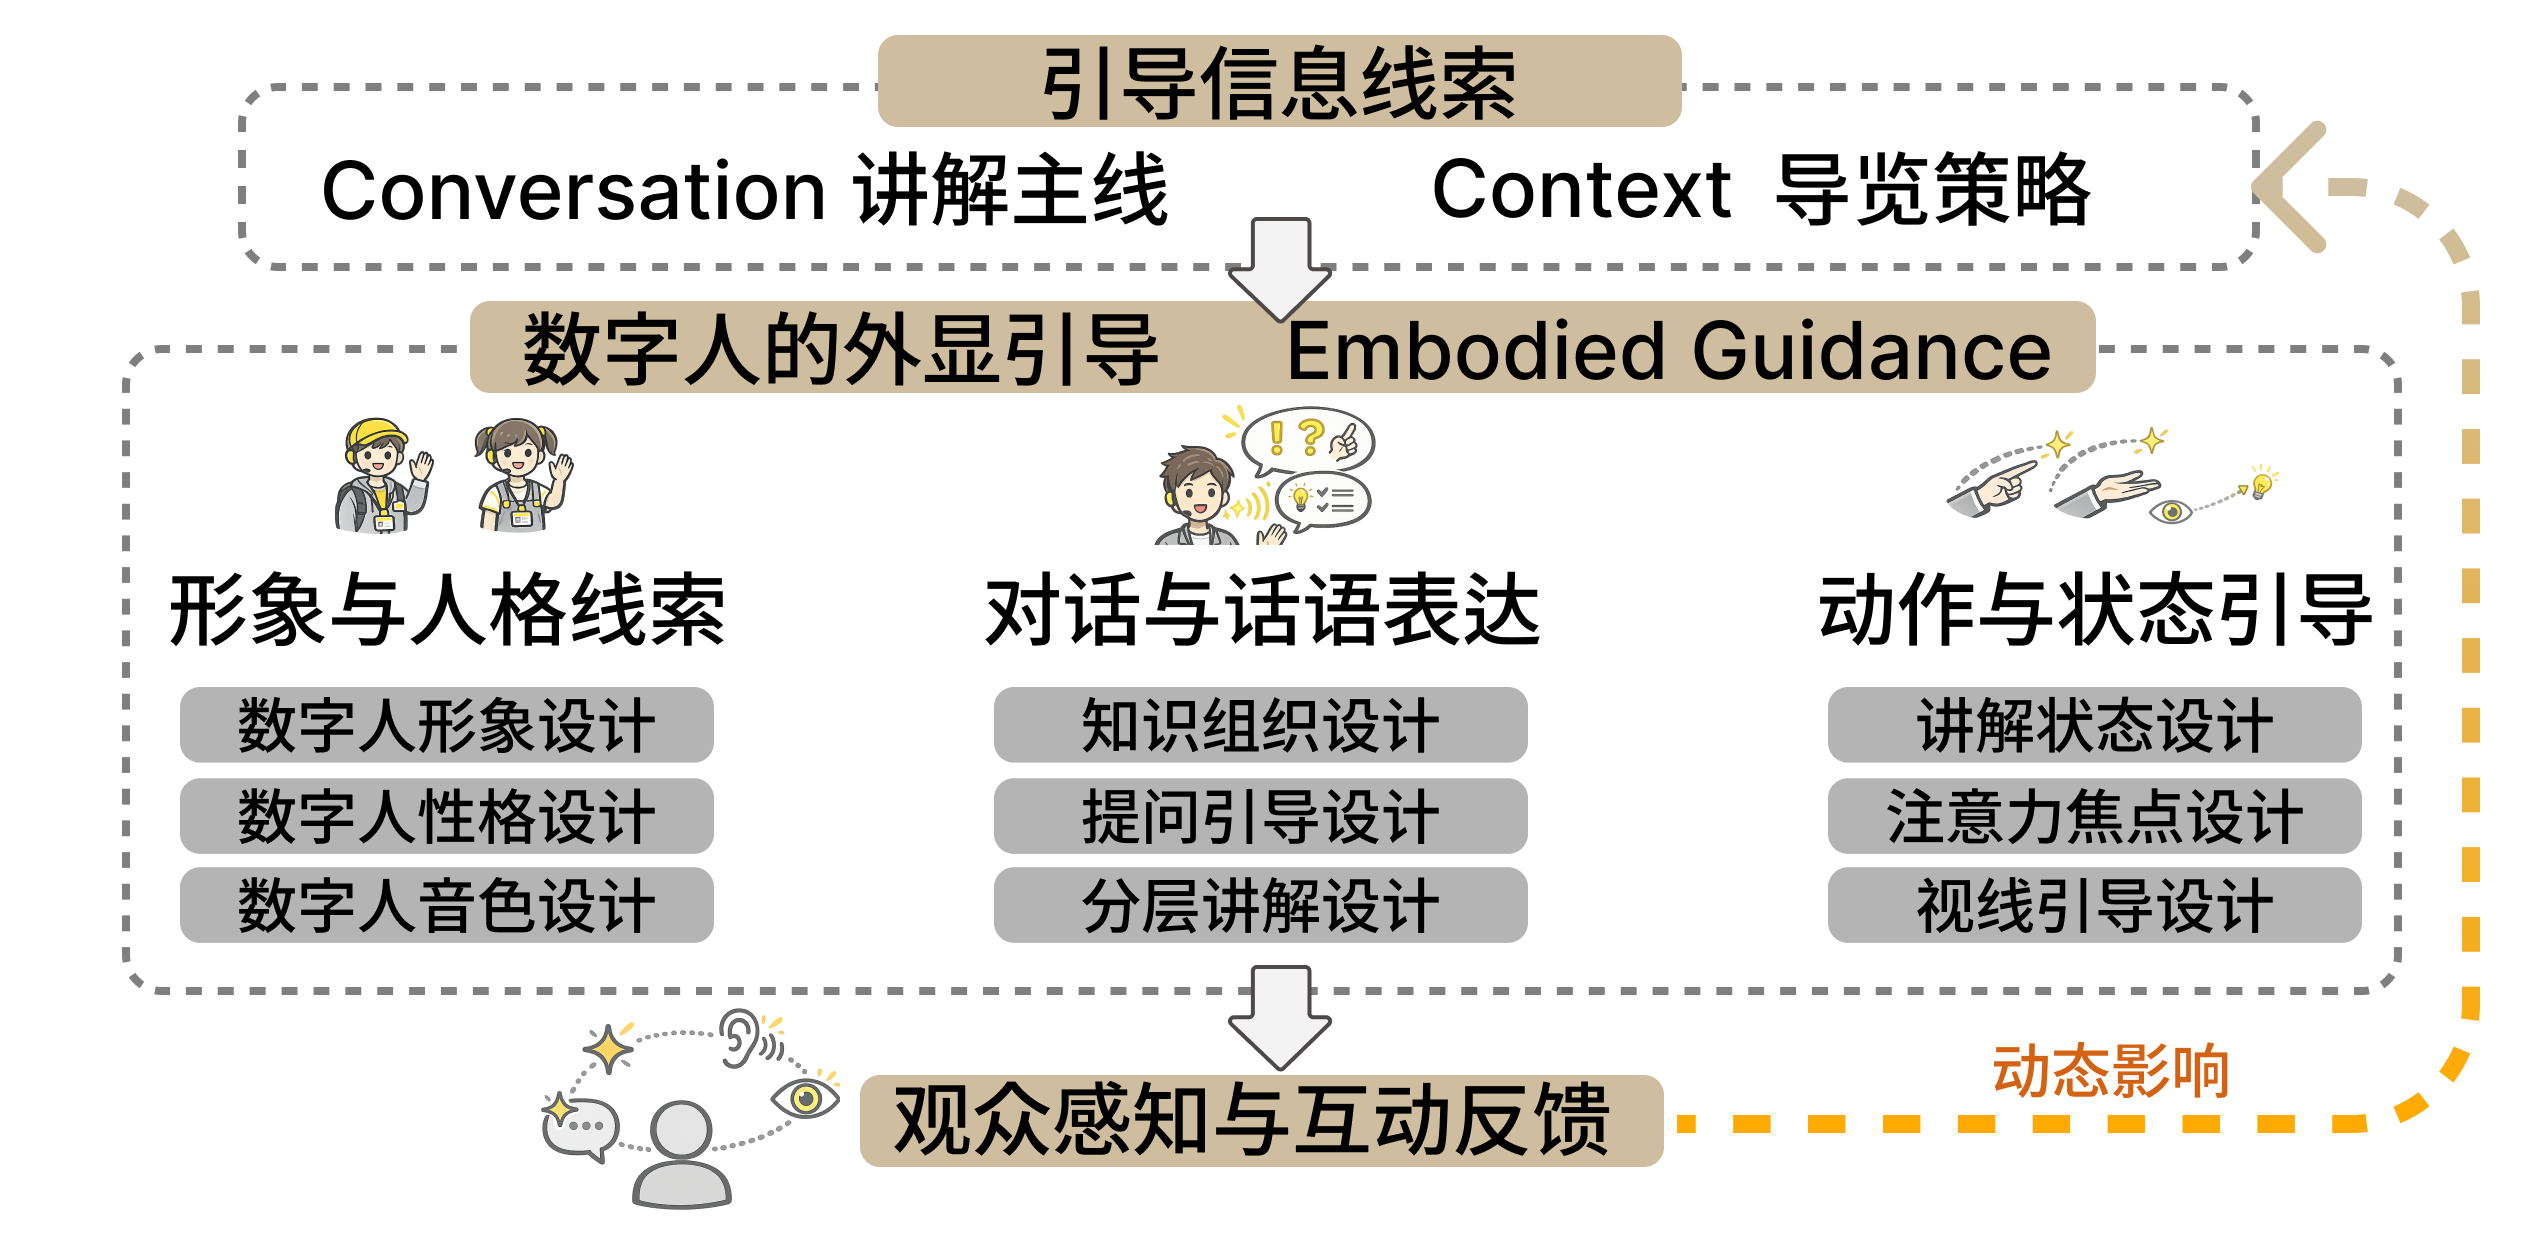
\includegraphics[width=\textwidth]{figure/figs/EG.png}
    \caption{面向导览感知的外显引导机制示意图}
    \label{fig-eg-mechanism}
\end{figure}

\par
这一层设计直接关系到导览体验是否真正成立。对于观众而言，参观过程中的理解常常依附于当下的观看方向、当前的讲解焦点以及交流节奏的连续展开。若系统只完成语义层面的组织，观众虽然能够接收到内容，却较难迅速把握当前该关注什么、何处值得停留、何时适合继续提问。外显引导机制的加入，使讲解重点获得清晰的感知入口，使空间方向获得可跟随的提示形式，也使交流状态获得可识别的展开方式。由此，导览从单纯的信息传递进一步发展为一种具有方向感、节奏感与现场感的引导过程。

从框架关系来看，外显引导承担着感知层转译的角色。叙事组织机制决定讲解如何展开，情境编排机制决定讲解围绕何种现场条件被组织，外显引导机制则让这些内部逻辑以数字人导览的方式显现在观众面前。观众看到数字人的站位、朝向、动作、神态，听到其语气、停顿与表达节奏，便能够快速形成对当前导览状态的判断：此刻处于介绍、强调、转场还是等待回应；眼前围绕的是整体背景、局部细节还是某个值得追问的线索；接下来适合继续观看、跟随移动还是进入互动。这样的感知组织，使导览获得更强的可进入性，也让系统的策略安排真正落到观众的参观行为中。

进一步看，外显引导还承担着连接观众反馈与后续导览策略的作用。观众的视线停留、跟随动作、回应频率与互动热度，会通过感知与互动反馈再次进入情境判断，推动情境编排机制对后续导览策略进行调整。由此，数字人的外显引导形成了一个持续运转的现场机制：前文生成的讲解主线与情境策略，经由数字人的外显表达进入观众感知；观众的感知与反馈又反过来参与下一步情境更新。这样的循环让导览呈现出更强的活性，也让数字人在场馆中拥有了接近真实引导者的现场组织能力。

\subsection{外显引导在数字人导览中的体现形式}
如图\ref{fig-eg-mechanism}所示，外显引导落实到数字人导览中，主要通过形象与人格呈现、语音与话语表达、动作与状态引导三类形式展开。这三类形式共同构成观众感知导览的主要入口，也共同塑造数字人在现场的引导存在感。

首先，形象与人格呈现为导览建立起稳定的在场关系。观众进入展厅后，面对数字人所形成的第一层判断，往往来自其角色气质、形象风格与交流姿态。导览员式的形象呈现能够迅速建立场景对应关系，让观众自然进入被带领、被陪伴的参观状态；人格线索则进一步影响导览体验的情绪氛围，例如亲和、沉稳、活泼、耐心等差异，会直接影响观众对数字人可信度、可接近性与交流意愿的感受。由此，形象与人格呈现承担着导览关系的开启功能，让观众能够较快完成角色识别，并在心理上接受这一导览媒介。

其次，语音与话语表达让讲解主线真正获得可感知的推进节奏。前文由叙事组织机制组织出的内容结构，需要借助数字人的语音语调、句式安排与话语节奏进入观众的理解过程。语速的快慢、停顿的位置、重音的分配、提问的方式、回应的衔接，都会直接影响观众对讲解重点的把握，也会影响其对导览节奏的体感。对观众而言，一段讲解是否易于跟上，某个重点是否足够鲜明，当前交流是否仍然留有继续进入的空间，往往都通过话语表达被感知。语音与话语表达由此承担着主线推进与交流组织的作用，使讲解从文本层的内容安排发展为现场中的节奏经验。

再次，动作与状态引导承担着空间组织与注意力调度的角色。导览发生在空间中，观众的视线、身体朝向与停留行为始终与讲解对象相互联动。数字人的视线指向、手势动作、转身幅度、停顿时机、等待姿态，都会向观众发出明确的引导提示：当前该看哪里，此刻强调何处，何时适合移动，何时适合继续听下去。尤其在展厅这样的开放场域中，动作与状态引导能够显著减轻观众在方向判断上的负担，让讲解对象、空间位置与当前语义重点形成更清晰的对应关系。由此，导览获得更强的可跟随性，观众也更容易在现场形成连续的注意力流动。

三类体现形式共同作用时，数字人的导览能力才真正完整显现。形象与人格呈现建立导览关系，语音与话语表达组织讲解推进，动作与状态引导完成空间中的方向提示与注意力调度。三者相互配合，使前文形成的讲解主线与情境策略进入观众的观看、聆听与互动过程，最终转化为一种具有现场感的引导体验。对于实际导览而言，这样的设计带来的价值十分直接：观众更容易识别当前重点，更容易跟上导览节奏，也更容易在合适时机进入互动；数字人则由内容承载者进一步发展为节奏组织者、空间提示者与交流推动者。导览体验因此呈现出更清晰的方向结构，也更贴近真实参观过程中对引导媒介的实际期待。


\section{本章小结}
本章围绕博物馆导览场景中对话式数字人的设计需求，提出并细化了面向博物馆导览的数字人智能交互设计框架。首先，基于前文对导览任务、场域特征与数字人展示问题的梳理，明确了叙事组织、情境编排与外显引导三个维度在导览过程中的必要性。随后，本文对框架进行了进一步细化：面向导览推进的叙事组织机制从导览内容的组织出发，处理讲解单元、导览路径与主线收束等问题；面向现场导览的情境编排机制围绕现场导览条件展开，组织参观者状态、空间位置与会话进程等情境线索；面向导览感知的外显引导机制则进一步将导览意图转化为数字人的外显设计，使讲解重点、空间方向与交流关系能够以可感知的方式被观众识别和跟随。

通过上述细化，面向博物馆导览的数字人智能交互设计框架被组织为一套面向博物馆导览的设计方法：面向导览推进的叙事组织机制负责讲解脉络的组织，面向现场导览的情境编排机制负责现场条件的判断与约束，面向导览感知的外显引导机制负责导览意图的外显与感知支撑。三者共同构成后续系统设计与实践实现的理论基础，也为下一章围绕系统架构、模块映射与设计实现的展开提供了结构依据。
